%!TEX root = ComputerScienceOne.tex

%Conditionals - exercises

\section{Exercises}

\begin{exer}
Write a program that prompts the user for an $x$ and a $y$ coordinate 
in the Cartesian plane and prints out a message indicating if the point 
$(x,y)$ lies on an axis ($x$ or $y$ axis, or both) or what quadrant it lies 
in (see Figure \ref{fig:Quadrants}).

\begin{figure}[h]
  \centering
 
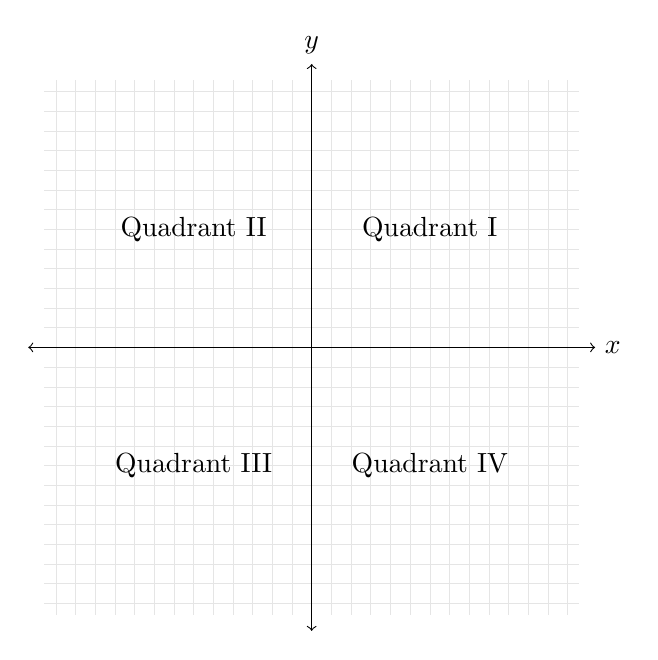
\begin{tikzpicture}
  \draw[step=.25cm,black!10!white,very thin] (-3.4,-3.4) grid (3.4,3.4); %
  \draw[<->] (-3.6,0) -- (3.6,0) node[right] {$x$};%
  \draw[<->] (0,-3.6) -- (0,3.6) node[above] {$y$};%
  \node at (1.5,1.5) {Quadrant I};
  \node at (-1.5,1.5) {Quadrant II};
  \node at (-1.5,-1.5) {Quadrant III};
  \node at (1.5,-1.5) {Quadrant IV};
  %\draw (0,0) circle (1cm);%
\end{tikzpicture}

 \caption{Quadrants of the Cartesian Plane}
 \label{fig:Quadrants}
\end{figure}
\end{exer}

\begin{exer}
A BOGO (Buy-One, Get-One) sale is a promotion in which a person buys two
items and receives a 50\% discount on the less expensive one.  Write a program
that prompts the user for the cost of two items, computes a 50\% discount
on the less expensive one, and then computes a grand total.
\end{exer}

\begin{exer}
Write a program that will calculate and print a bill for the city power
company.  The rates vary depending on whether the use is residential,
commercial, or industrial.  The program should prompt the user to 
indicate which type the customer is as well as a total kilowatt hour (kWh)
used and compute the total based on the rates in Table \ref{table:kwhRates}.

\begin{table}[h]
\centering
\begin{tabular}{l|c|c}
\hline
Type & Base & Rate \\
\hline\hline
Residential & \$24.50 & \$0.1415 per kWh \\
Commercial & \$75.00 & \$0.1750 per kWh \\
Industrial & \$245.00 & \$0.2774 per kWh
\end{tabular}
\caption{Rates per kWh for each type of customer}
\label{table:kwhRates}
\end{table}

Each customer is assessed a \emph{base} cost of service regardless of how
much electricity they use.  In addition, if industrial customers use more than 
2000 kWh, they are assessed an additional \$0.05 per kWh.
\end{exer}

%\begin{exer}
%Write a program to compute the federal income tax liability for a married couple 
%filing jointly based on their Adjusted Gross Income (AGI) which is presented in
%Table \ref{table:taxBrackets}.
%
%\begin{table}[h]
%\centering
%\begin{tabular}{|l|l|p{.5\textwidth}|}
%\hline
%AGI is over & But not over & Tax \\
%\hline\hline
%-- & \$18,150 & 10\% of the AGI\\
%\hline
%\$18,150 & \$73,800 & \$1,815 plus 15\% of the AGI in excess of \$18,150\\
%\hline
%\$73,800 & \$148,850 & \$10,162.50 plus 25\% of the AGI in excess of \$73,800\\
%\hline
%\$148,850 & \$225,850 & \$28,925 plus 28\% of the AGI in excess of \$148,850\\
%\hline
%\$225,850 & \$405,100 & \$50,765 plus 33\% of the AGI in excess of \$225,850\\
%\hline
%\$405,100 & \$457,600 & \$109,587.50 plus 35\% of the AGI in excess of \$405,100\\
%\hline
%\$457,600 & --- & \$127,962.50 plus 39.6\% of the AGI in excess of \$457,600\\
%\hline
%\end{tabular}
%\caption{2014 Tax Brackets for Married Couples Filing Jointly}
%\label{table:taxBrackets}
%\end{table}
%
%In addition, tax payers can take a tax credit (that offsets their tax liability) if they 
%have qualifying children.  The rules are as follows:
%\begin{itemize}
%  \item If the AGI is \$110,000 or more, they cannot claim a credit (the credit is \$0)
%  \item Each child is worth \$1,000 credit, however at most \$3,000 can be claimed
%  \item The credit is not refundable: if the credit results in a negative tax liability, the tax liability is simply \$0
%\end{itemize}
%
%As an example: suppose that a couple has \$35,000 AGI and has two children.  Their tax liability is
%$$\$1,815 + 0.15 \times (\$35,000 - \$18,150) = \$4,342.50$$
%However, the two children represent a \$2,000 refund, so their total tax liability would be \$2,342.50.
%
%Write a program that prompts a user for an AGI and a number of children and computes
%the total tax liability based on the rules above.
%\end{exer}

\begin{exer}

Various substances have different boiling points.  A selection of
substances and their boiling points can be found in Table \ref{table:boilingPoints}.
Write a program that prompts the user for the observed boiling point of
a substance in degrees Celsius and identifies the substance if the
observed boiling point is within 5\% of the expected boiling point.  If
the data input is more than 5\% higher or lower than any of the boiling
points in the table, it should output \texttt{Unknown substance}.

\begin{table}[h]
  \centering
  \begin{tabular}{ll}
    \textbf{Substance} & \textbf{Boiling Point (C)} \\
    \hline
    Methane & -161.7 \\
    Butane & -0.5 \\
    Water & 100 \\
    Nonane & 150.8 \\
    Mercury & 357 \\
    Copper & 1187 \\
    Silver & 2193 \\
    Gold & 2660 \\
    \hline
  \end{tabular}
\caption{Expected Boiling Points}
\label{table:boilingPoints}
\end{table}
\end{exer}

\begin{exer}
Electrical resistance in various metals can be measured using nano-ohm metres ($n\Omega\cdot m$).
Table \ref{table:resistivity} gives the resistivity of several metals.

\begin{table}[h]
\centering
\begin{tabular}{|l|l|}
\hline
Material & Resistivity ($n\Omega\cdot m$) \\
\hline\hline
Copper & 16.78 \\
\hline
Aluminum & 26.50\\
\hline
Beryllium & 35.6 \\
\hline
Potassium & 72.0 \\
\hline
Iron & 96.10 \\
\hline
\end{tabular}
\caption{Resistivity of several metals}
\label{table:resistivity}
\end{table}

Write a program that prompts the user for an observed resistivity of an unknown material (as nano-ohm metres)
and identifies the substance if the observed resistivity is within $\pm3\%$ of the known resistivity of any of the materials
in Table \ref{table:resistivity}.  If the input value lies outside the $\pm 3\%$ range, output \texttt{Unknown substance}.
\end{exer}

\begin{exer}
The visible light spectrum is measured in nanometer (nm) frequencies.  Ranges roughly correspond to 
visible colors as depicted in Table \ref{table:lightSpectrum}.

\begin{table}[h]
\centering
\begin{tabular}{|c|c|}
\hline
Color & Wave length range (nm) \\
\hline
\hline
Violet &  380 -- 450 \\
\hline
Blue & 450 -- 475 \\
\hline
Indigo & 476 -- 495 \\
\hline
Green & 495 -- 570 \\
\hline
Yellow & 570 -- 590 \\
\hline
Orange & 590 -- 620 \\
\hline
Red & 620 - 750\\
\hline
\end{tabular}
\caption{Visible Light Spectrum Ranges}
\label{table:lightSpectrum}
\end{table}
Write a program that takes an integer corresponding to a wavelength and 
outputs the corresponding color.  If the value lies outside the ranges it should 
output \texttt{Not a visible wavelength}.  If a value lies within multiple color 
ranges it should print all that apply (for example, a wavelength of 495 is 
``Indigo-green'').
\end{exer}

\begin{exer}
A certain production of steel is graded according to the following conditions:
\begin{enumerate}
  \item[(i)] Hardness must be greater than 50
  \item[(ii)] Carbon content must be less than 0.7
  \item[(iii)] Tensile strength must be greater than 5600
\end{enumerate}
A grade of 5 thru 10 is is assigned to the steel according to the conditions in Table \ref{table:steelGrades}.
\begin{table}[h]
\centering
\begin{tabular}{|c|l|}
\hline
Grade & Conditions \\
\hline
\hline
10 & All three conditions are met \\
\hline
9   & Conditions (i) and (ii) are met \\
\hline
8  & Conditions (ii) and (iii) are met\\
\hline
7  & Conditions (i) and (iii) are met \\
\hline
6 & If only 1 of the three conditions is met \\
\hline
5  & If none of the conditions are met \\
\hline
\end{tabular}
\caption{Grades of Steel}
\label{table:steelGrades}
\end{table}
Write a program that will read in the hardness, carbon content, and tensile strength as inputs and output the 
corresponding grade of the steel.
\end{exer}

\begin{exer}
A triangle can be characterized in terms of the length of its three sides.  In particular, an \emph{equilateral}
triangle is a triangle with all three sides being equal.  A triangle such that two sides have the same length 
is \emph{isosceles} and a triangle with all three sides having a different length is \emph{scalene}.  Examples
of each can be found in Figure \ref{figure:triangleTypes}.

In addition, the three sides of a triangle are \emph{valid} only if the sum of any two sides is strictly greater 
than the third length.

Write a program to read in three numbers as the three sides of a triangle.  If the three sides do not
form a valid triangle, you should indicate so.  Otherwise, if valid, your program should output whether or
not the triangle is equilateral, isosceles or scalene.

\begin{figure}[h]
\centering
\subfigure[Equilateral Triangle]{
~~~~~~\includegraphics[scale=0.25]{images/200px-Triangle-Equilateral.png}~~~~~~
}
\subfigure[Isosceles Triangle]{
~~~~~~\includegraphics[scale=0.20]{images/200px-Triangle-Isosceles.png}~~~~~~
}
\subfigure[Scalene Triangle]{
~~~~\includegraphics[scale=0.50]{images/200px-Triangle-Scalene.png}~~~~
}
\caption{Three types of triangles}
\label{figure:triangleTypes}
\end{figure}

\end{exer}

\begin{exer}
Body Mass Index (BMI) is a healthy statistic based on a person's mass and height.  For a healthy adult male
BMI is calculated as 
 $$\mathrm{BMI} = \frac{m}{h^2} \cdot 703.069579$$
where $m$ is the person's mass (in lbs) and $h$ is the person's height (in whole inches).  Write a program
that reads in a person's mass and height as input and outputs a characterization of the person's health with
respect to the categories in Table \ref{table:bmiCategories}.
\begin{table}[h]
\centering
\begin{tabular}{|l|l|}
\hline
Range & Category \\
\hline
\hline
$\mathrm{BMI} < 15$ & Very severely underweight \\
\hline
$15 \leq \mathrm{BMI} < 16$ & Severely underweight \\
\hline
$16 \leq \mathrm{BMI} < 18.5$ & Underweight \\
\hline
$18.5 \leq \mathrm{BMI} < 25$ & Normal \\
\hline
$25 \leq \mathrm{BMI} < 30$ & Overweight \\
\hline
$30 \leq \mathrm{BMI} < 35$ & Obese Class I \\
\hline
$35 \leq \mathrm{BMI} < 40$ & Obese Class II \\
\hline
$\mathrm{BMI} \geq 40$ & Obese Class III \\
\hline
\end{tabular}
\caption{BMI Categories}
\label{table:bmiCategories}
\end{table}
\end{exer}

\begin{exer}
Let $R_1$ and $R_2$ be rectangles in the plane defined as follows.  Let $(x_1, y_1)$ be
point corresponding to the lower-left corner of $R_1$ and let $(x_2, y_2)$ be the point of its
upper-right corner.  Let $(x_3, y_3)$ be point corresponding to the lower-left corner of $R_2$
and let $(x_4, y_4)$ be the point of its upper-right corner.

Write a program to determine the \emph{intersection} of these two rectangles.  In general,
the intersection of two rectangles is another rectangle.  However, if the two rectangles abut each
other, the intersection could be a horizontal or vertical line segment (or even a point).  It is also possible that the
intersection is \emph{empty}.  Your program will need to distinguish between these cases.

If the intersection of $R_1, R_2$ is a rectangle, $R_3$, your program should output two
points (the lower-left and upper-right corners of $R_3$) as well as the \emph{area} of $R_3$.
If the intersection is a line segment, your program should output the two \emph{end-points}
and whether it is a vertical or horizontal line segment.  Finally, if the intersection is empty your
program should output ``empty intersection''.  Your program should also be robust enough to
check that the input is valid (it should not accept empty or ``reversed'' rectangles).

Your program should read in $x_1, y_1, x_2, y_2, x_3, y_3, x_4, y_4$ from the user and
perform the computation above.  As an example, the values  $2, 1, 6, 7.5, 4, 5.5, 8.5, 8.25$
would correspond to the two rectangles in Figure \ref{fig:rectangleIntersection}.

\begin{figure}
\centering

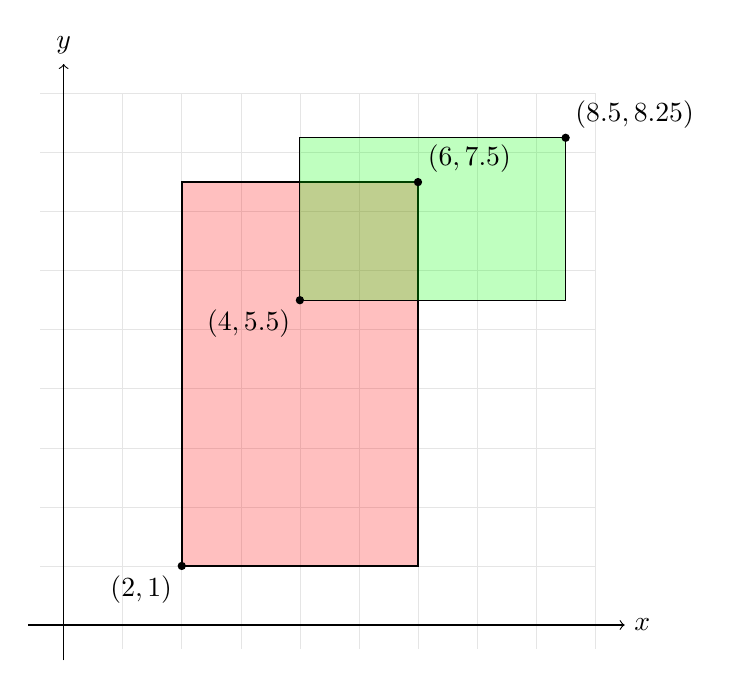
\begin{tikzpicture}[scale=0.75]
  \draw[step=1.0cm,black!10!white,very thin] (-0.4,-0.4) grid (9,9); %
  \draw[->] (-0.6,0) -- (9.5,0) node[right] {$x$};%
  \draw[->] (0,-0.6) -- (0,9.5) node[above] {$y$};%

  \filldraw[fill=red,thick,fill opacity=.25] (2, 1) rectangle (6, 7.5);
  \filldraw[fill=green,fill opacity=.25] (4, 5.5) rectangle (8.5, 8.25);

  \fill (2, 1) circle (2pt);
  \fill (6, 7.5) circle (2pt);
  \fill (4, 5.5) circle (2pt);
  \fill (8.5, 8.25) circle (2pt);

  \node [] (A) at (2, 1) [below left] {$(2, 1)$};
  \node [] (B) at (6, 7.5) [above right] {$(6, 7.5)$};
  \node [] (C) at (4, 5.5) [below left] {$(4, 5.5)$};
  \node [] (D) at (8.5, 8.25) [above right] {$(8.5, 8.25)$};

\end{tikzpicture}

\caption{Intersection of Two Rectangles}
\label{fig:rectangleIntersection}
\end{figure}

The output for this instance should look something like the following.

\begin{minted}{text}
Intersecting rectangle: (4, 5.5), (6, 7.5)
Area: 4.00
\end{minted}
\end{exer}

\begin{exer}
Write an app to help people track their cell phone usage.  Cell 
phone plans for this particular company give you a certain number of minutes
every 30 days which must be used or they are lost (no rollover).  We want
to track the average number of minutes used per day and inform the user
if they are using too many minutes or can afford to use more.

Write a program that prompts the user to enter the following pieces of data:
\begin{itemize}
  \item Number of minutes in the plan per 30 day period, $m$
  \item The current day in the 30 day period, $d$
  \item The total number of minutes used so far $u$
\end{itemize}
The program should then compute whether the user is over, under, or 
right on the average daily usage under the plan.  It should also inform
them of how many minutes are left and how many, on average, they can
use per day for the rest of the month.  Of course, if they've run out of minutes, it
should inform them of that too.

For example, if the user enters $m = 250$, $d = 10$, and $u = 150$, your
program should print out something similar to the following.

\begin{minted}{text}
10 days used, 20 days remaining
Average daily use: 15 min/day

You are EXCEEDING your average daily use (8.33 min/day), 
continuing this high usage, you'll exceed your minute plan by
200 minutes.

To stay below your minute plan, use no more than 5 min/day.
\end{minted}

Of course, if the user is under their average daily use, a different
message should be presented.  You are allowed/encouraged to 
compute any other stats for the user that you feel would be useful.
\end{exer}

\begin{exer}
Write a program to  help a floor tile company determine how many
tiles they need to send to a work site to tile a floor in a room.  For 
simplicity, assume that all rooms are perfectly rectangular with no 
obstructions; we will also omit any additional measurements related 
to grouting.  

Further, we will assume that all tile is laid in a grid pattern centered 
at the center of the room.  That is, four tiles will meet at their corners 
at the center of the room with tiles laid out to the edge of the room.  
Thus, it may be the case that the final row and/or column at the edge 
may need to be cut.  Also note that if the cut is short enough, the 
remaining tile can be used on the other end of the room (same goes 
for the corners).

The program will take the following input:
\begin{itemize}
  \item $w$ - the width of the room
  \item $l$ - the length of the room
  \item $t$ - width/length of the tile (all tiles are perfectly square)
\end{itemize}

If we can use whole tiles to perfectly fit the room, then we do so.  
For example, on the input $(10, 10, 1)$, we could perfectly tile a 
$10 \times 10$ room with 100 $1 \times 1$ tiles.  If the tiles don't 
perfectly fit, then we have to consider the possibility of waste 
and/or reuse.  Consider the examples in Figure \ref{figure:floorTiling}.

\begin{figure}
\centering

\subfigure[Example 1] {
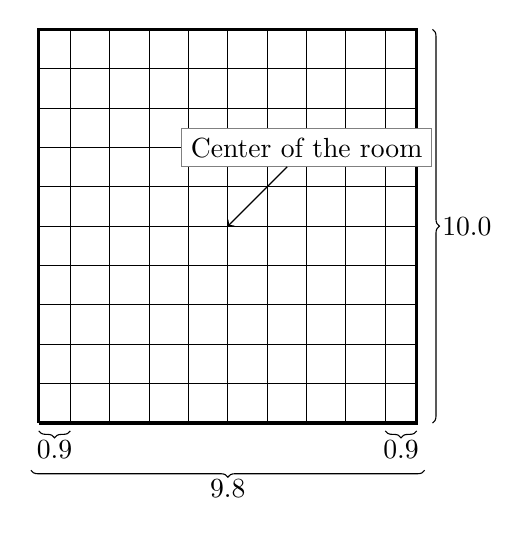
\begin{tikzpicture}[scale=.5]

\draw[step=1cm] (-4.8, -5) grid (4.8, 5);

\draw[very thick] (-4.8, -5) -- (4.8, -5) -- (4.8, 5) -- (-4.8, 5) -- (-4.8, -5);

\draw[decorate,decoration={brace,mirror}] (-4.8, -5.2) -- (-4, -5.2) node[midway,below] {0.9};
\draw[decorate,decoration={brace,mirror}] (4, -5.2) -- (4.8, -5.2) node[midway,below] {0.9};

\draw[decorate,decoration={brace,mirror}] (-5, -6.2) -- (5, -6.2) node[midway,below] {9.8};

\draw[decorate,decoration={brace,mirror}] (5.2, -5) -- (5.2, 5)  node [midway,right] {10.0};

\node (A) at (2,2) [rectangle,draw=black!50,fill=white] {Center of the room};
\draw[->] (A) -- (0,0);
\end{tikzpicture}
}
\subfigure[Example 2] {
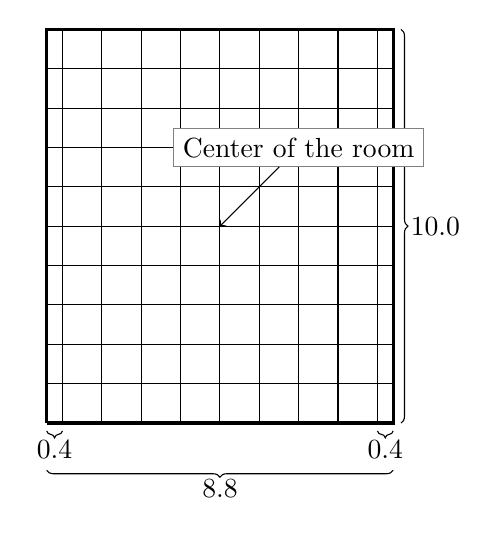
\begin{tikzpicture}[scale=.5]

\draw[step=1cm] (-4.4, -5) grid (4.4, 5);

\draw[very thick] (-4.4, -5) -- (4.4, -5) -- (4.4, 5) -- (-4.4, 5) -- (-4.4, -5);

\draw[decorate,decoration={brace,mirror}] (-4.4, -5.2) -- (-4, -5.2) node[midway,below] {0.4};
\draw[decorate,decoration={brace,mirror}] (4, -5.2) -- (4.4, -5.2) node[midway,below] {0.4};

\draw[decorate,decoration={brace,mirror}] (-4.4, -6.2) -- (4.4, -6.2) node[midway,below] {8.8};

\draw[decorate,decoration={brace,mirror}] (4.6, -5) -- (4.6, 5)  node [midway,right] {10.0};

\node (A) at (2,2) [rectangle,draw=black!50,fill=white] {Center of the room};
\draw[->] (A) -- (0,0);
\end{tikzpicture}
}
\caption{Examples of Floor Tiling}
\label{figure:floorTiling}
\end{figure}


The first example is from the input $(9.8, 100, 1)$.  In this case, 
we lay the tiles from the center of the room (8 full tile lengths) but 
are left with $0.9$ on either side.  If we cut a tile to fit the left
side, we are left with only $.1$ tile which is too short for the right 
side.  Therefore, we are forced to waste the $0.1$ length and cut 
a full tile for the right side.  In all, 100 tiles are required.

The second example is from the input $(8.8, 100, 1)$.  In this case, 
we again lay tiles from the center of the room (8 full tile lengths) and 
are left with $0.4$ lengths on either side.  Here, we \emph{can}
reuse the cut tile: cut a tile on one side $0.4$ with $0.6$ remaining, 
and cut $0.4$ on the other side of the tile (with the center $0.2$ 
length of the tile being waste).  Thus, both sides can be tiled with 
a single tile, meaning only 90 full tiles are needed to tile this room.

You may further assume that tiles used on 
the length-side end of the room \emph{cannot} be used to tile the 
width-side of the room (and vice versa).  Your program will compute 
and output the number of tiles required.
\end{exer}


